\section{Exercice 1 - Compteur de 2 bits}

Le but de cet exercice est de modéliser un compteur synchrone à 2 bits. Celui-ci utilisera une horloge et un un signal de reset synchrone. Ces deux fonctionnalités seront implémentées respectivement sur \textbf{PB\_0} et \textbf{PB\_1} qui sont des boutons poussoirs. L'affichage de sortie se fera sur \textbf{LED\_10} qui est un ensemble de deux leds.

\medskip

\noindent La modélisation respectera 2 conditions :
\begin{itemize}
  \item Le front montant de l’horloge est le front actif.
  \item Le reset est actif au niveau bas (\textbf{PB\_1 = '1'})
\end{itemize}
Ainsi, à chaque pression sur le bouton poissoir \textbf{PB\_0}, les LEDs afficheront successivement : '00', '01', '10', '11', '00', '01', etc. Si \textbf{PB\_1} est pressé puis \textbf{PB\_0}, le compteur sera réinitialisé à 0.

\subsection{Ports utilisés}

Au préalable, nous avons décommenté les lignes du fichier \textbf{carte\_tp.ucf} correspondant aux ports utilisés :
\textcode{Fichier : carte\_tp.ucf}
\begin{lstlisting}
NET "LED_10<0>"     LOC = "P44"     | IOSTANDARD = LVCMOS33;
NET "LED_10<1>"     LOC = "P51"     | IOSTANDARD = LVCMOS33;
NET "PB_0"          LOC = "P128"    | IOSTANDARD = LVCMOS33 | CLOCK_DEDICATED_ROUTE = FALSE;
NET "PB_1"          LOC = "P141"    | IOSTANDARD = LVCMOS33 | CLOCK_DEDICATED_ROUTE = FALSE;
\end{lstlisting}

\subsection{VHDL}

Nous proposons une modélisation VHDL de type \textbf{comportementale} puisque c'est plus simple à écrire et parfaitement adapté à notre besoin. En effet nous souhaitons utiliser \textbf{PROCESS} (instructions séquentielles). Les \textbf{signaux déclencheurs} du \textbf{PROCESS} seront les deux boutons poussoirs. Les deux LED permettent \og d'afficher\fg{} 4 valeurs décimales :
\begin{itemize}
  \item 0 soit 00 en binaire sur 2 bits
  \item 1 soit 01 en binaire sur 2 bits
  \item 2 soit 10 en binaire sur 2 bits
  \item 3 soit 11 en binaire sur 2 bits
\end{itemize}
Voici l'implémentation :

\textcode{Fichier : tp2\_1.vhd}
\vhdl
\begin{lstlisting}
entity tp2_1 is
  PORT(LED_10 : out integer range 0 to 3; -- la led peut afficher 4 valeurs sur 2 bits
        PB_0 : in bit;
        PB_1 : in bit); 
end tp2_1;

architecture Behavioral of tp2_1 is
begin
	process(PB_0,PB_1)
	variable i : integer range 0 to 3 := 0; -- variable qui sert d'alias du signal
	begin
		if (PB_1 = '1') then
			i := 0; -- dès que PB_1 est enfoncé, on reset
		elsif(PB_0'event AND PB_0='1') then
			i := i + 1; -- on incrémente à chaque pression de PB_0
		end if;
		LED_10 <= i; -- on affecte la valeur de la variable au signal
	end process;
end Behavioral;
\end{lstlisting}

\subsection{Synthèse}

\noindent On synthétise notre circuit :
\begin{figure}[!h]
   \centering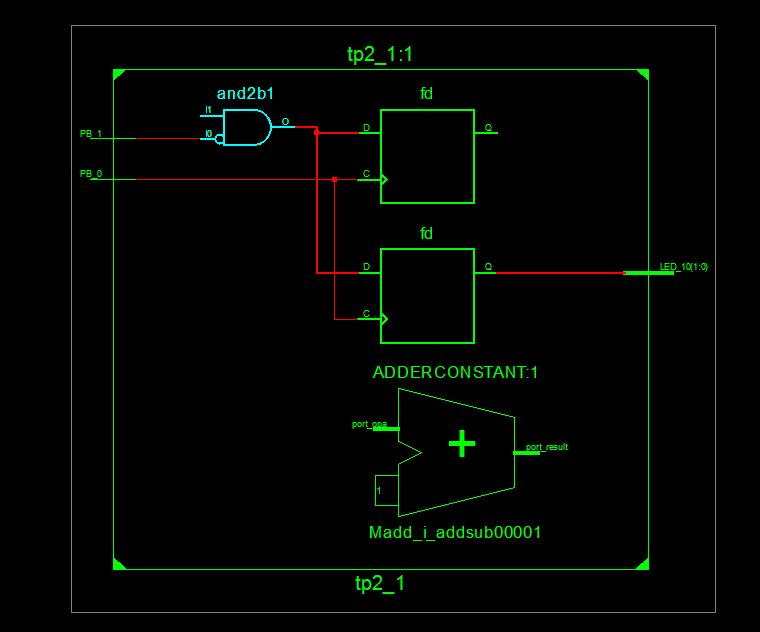
\includegraphics[width=0.95\textwidth]{files/tp2_1/RTL.png}
   \caption{Schéma \og RTL\fg{}}
\end{figure}

On constate que le synthétiseur a utilisé un circuit additionneur avec peu de portes. C'est un circuit \og pré-optimisé\fg{}, indépendant du FPGA cible. C'est une représentation logique du VHDL.

\begin{figure}[!h]
   \centering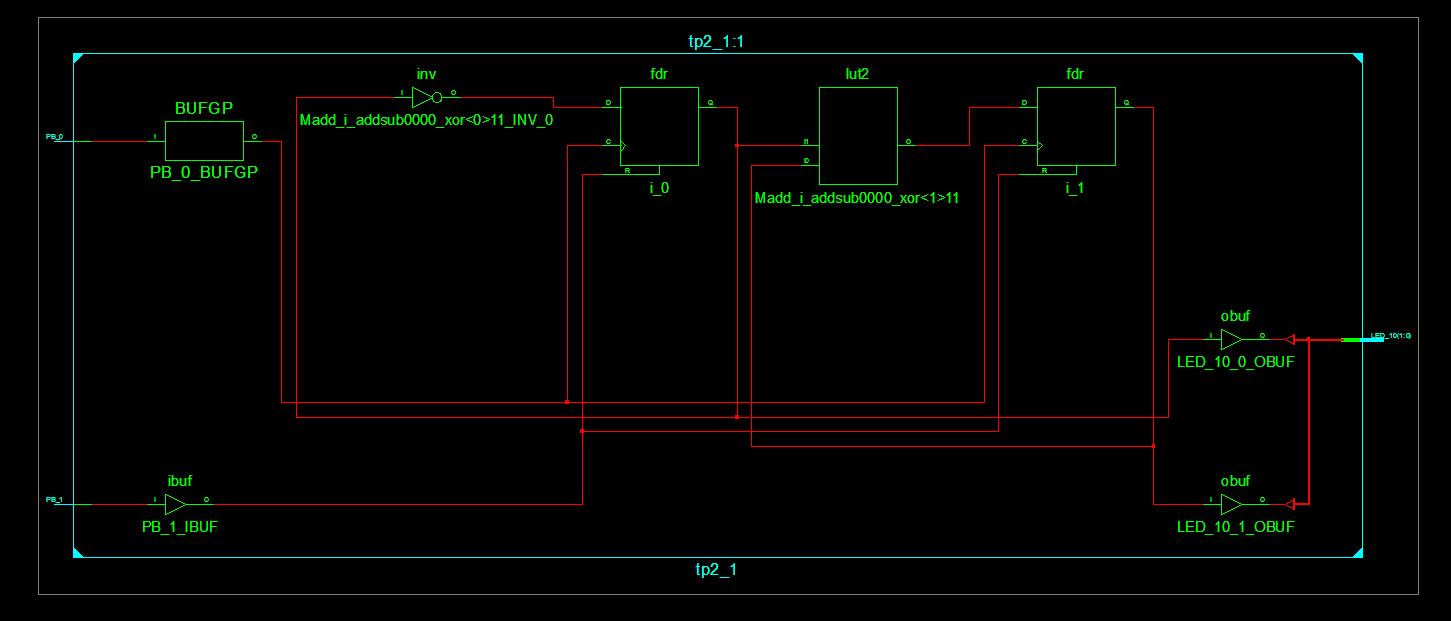
\includegraphics[width=\textwidth]{files/tp2_1/Tech.png}
   \caption{Schéma \og Technology\fg{}}
\end{figure}

Le schéma \og Technology\fg{} présente plus d'éléments que le schéma précédent (\textit{inv}, \textit{fdr}, etc) et est par conséquent beaucoup plus complexe. Ce schéma est généré après l'optimisation, qui est faite en fonction du FPGA cible. Les composants sont choisis selon ce FPGA cible. C'est une représentation technologique du VHDL optimisé.

\subsection{Simulation}

Après la synthèse, on simule notre circuit pour vérifier qu'il respecte le cahier des charges :

\begin{figure}[!h]
   \centering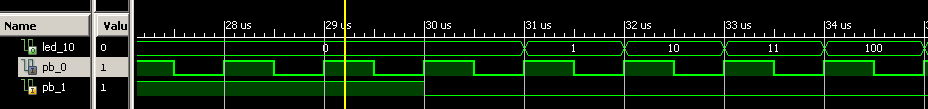
\includegraphics[width=\textwidth]{files/tp2_1/simulateur.png}
   \caption{Simulation}
\end{figure}

La simulation est correcte, nous avons bien un compteur incrémenté suivant l'horloge, qui est réinitialisé par le signal de reset (de façon synchrone avec le signal horloge\footnote{Pour reset notre compteur, il faut que le bouton reset soit actif (\textbf{PB\_1 = '1'}) lors du front d'horloge. En pratique, l'horloge est simulée à l'aide d'un bouton poussoir, de ce fait il fait garder le reset enfoncé (\textbf{PB\_1}) puis appuyer sur le bouton d'horloge (\textbf{PB\_0})}). En effet, au début du schéma, on constate que tant que \textbf{PB\_1} est \og enfoncé\fg{} (équivalent à 1), la valeur des LED est 0. Puis, lorsque le bouton poussoir est relâché (à partir de 30$\mu$s), la valeur affichée par les LED s'incrémente (01, 10, 11, 00, 01, etc).

\bigskip

Pour terminer on programme le FPGA avec notre code pour tester en pratique le bon fonctionnement. Après tests, notre programme est fonctionnel. On constatera que le reset est ici à nouveau synchrone.

\newpage